\section{Unwanted Heterogeneity}

There is no obvious pattern for different stations in epicentral distance and depth. This effect make the parameters calibration process, extremely difficult. The reason for that is unwanted heterogeneity. As we can see from the results, the element updating process impose unwanted heterogeneity. This happens because elements are updated based on their individual strain history. Therefore, studying individual stations will not lead to accurate results. Some of these stations provides very good match and some other provides not accurate results. Therefore, we take a look at maximum horizontal peak ground velocity to see if in general we can see the similarity. Fig.~\ref{fig:plane_lin_nonlin_eqlin}

\begin{figure}[H]
    \centering
    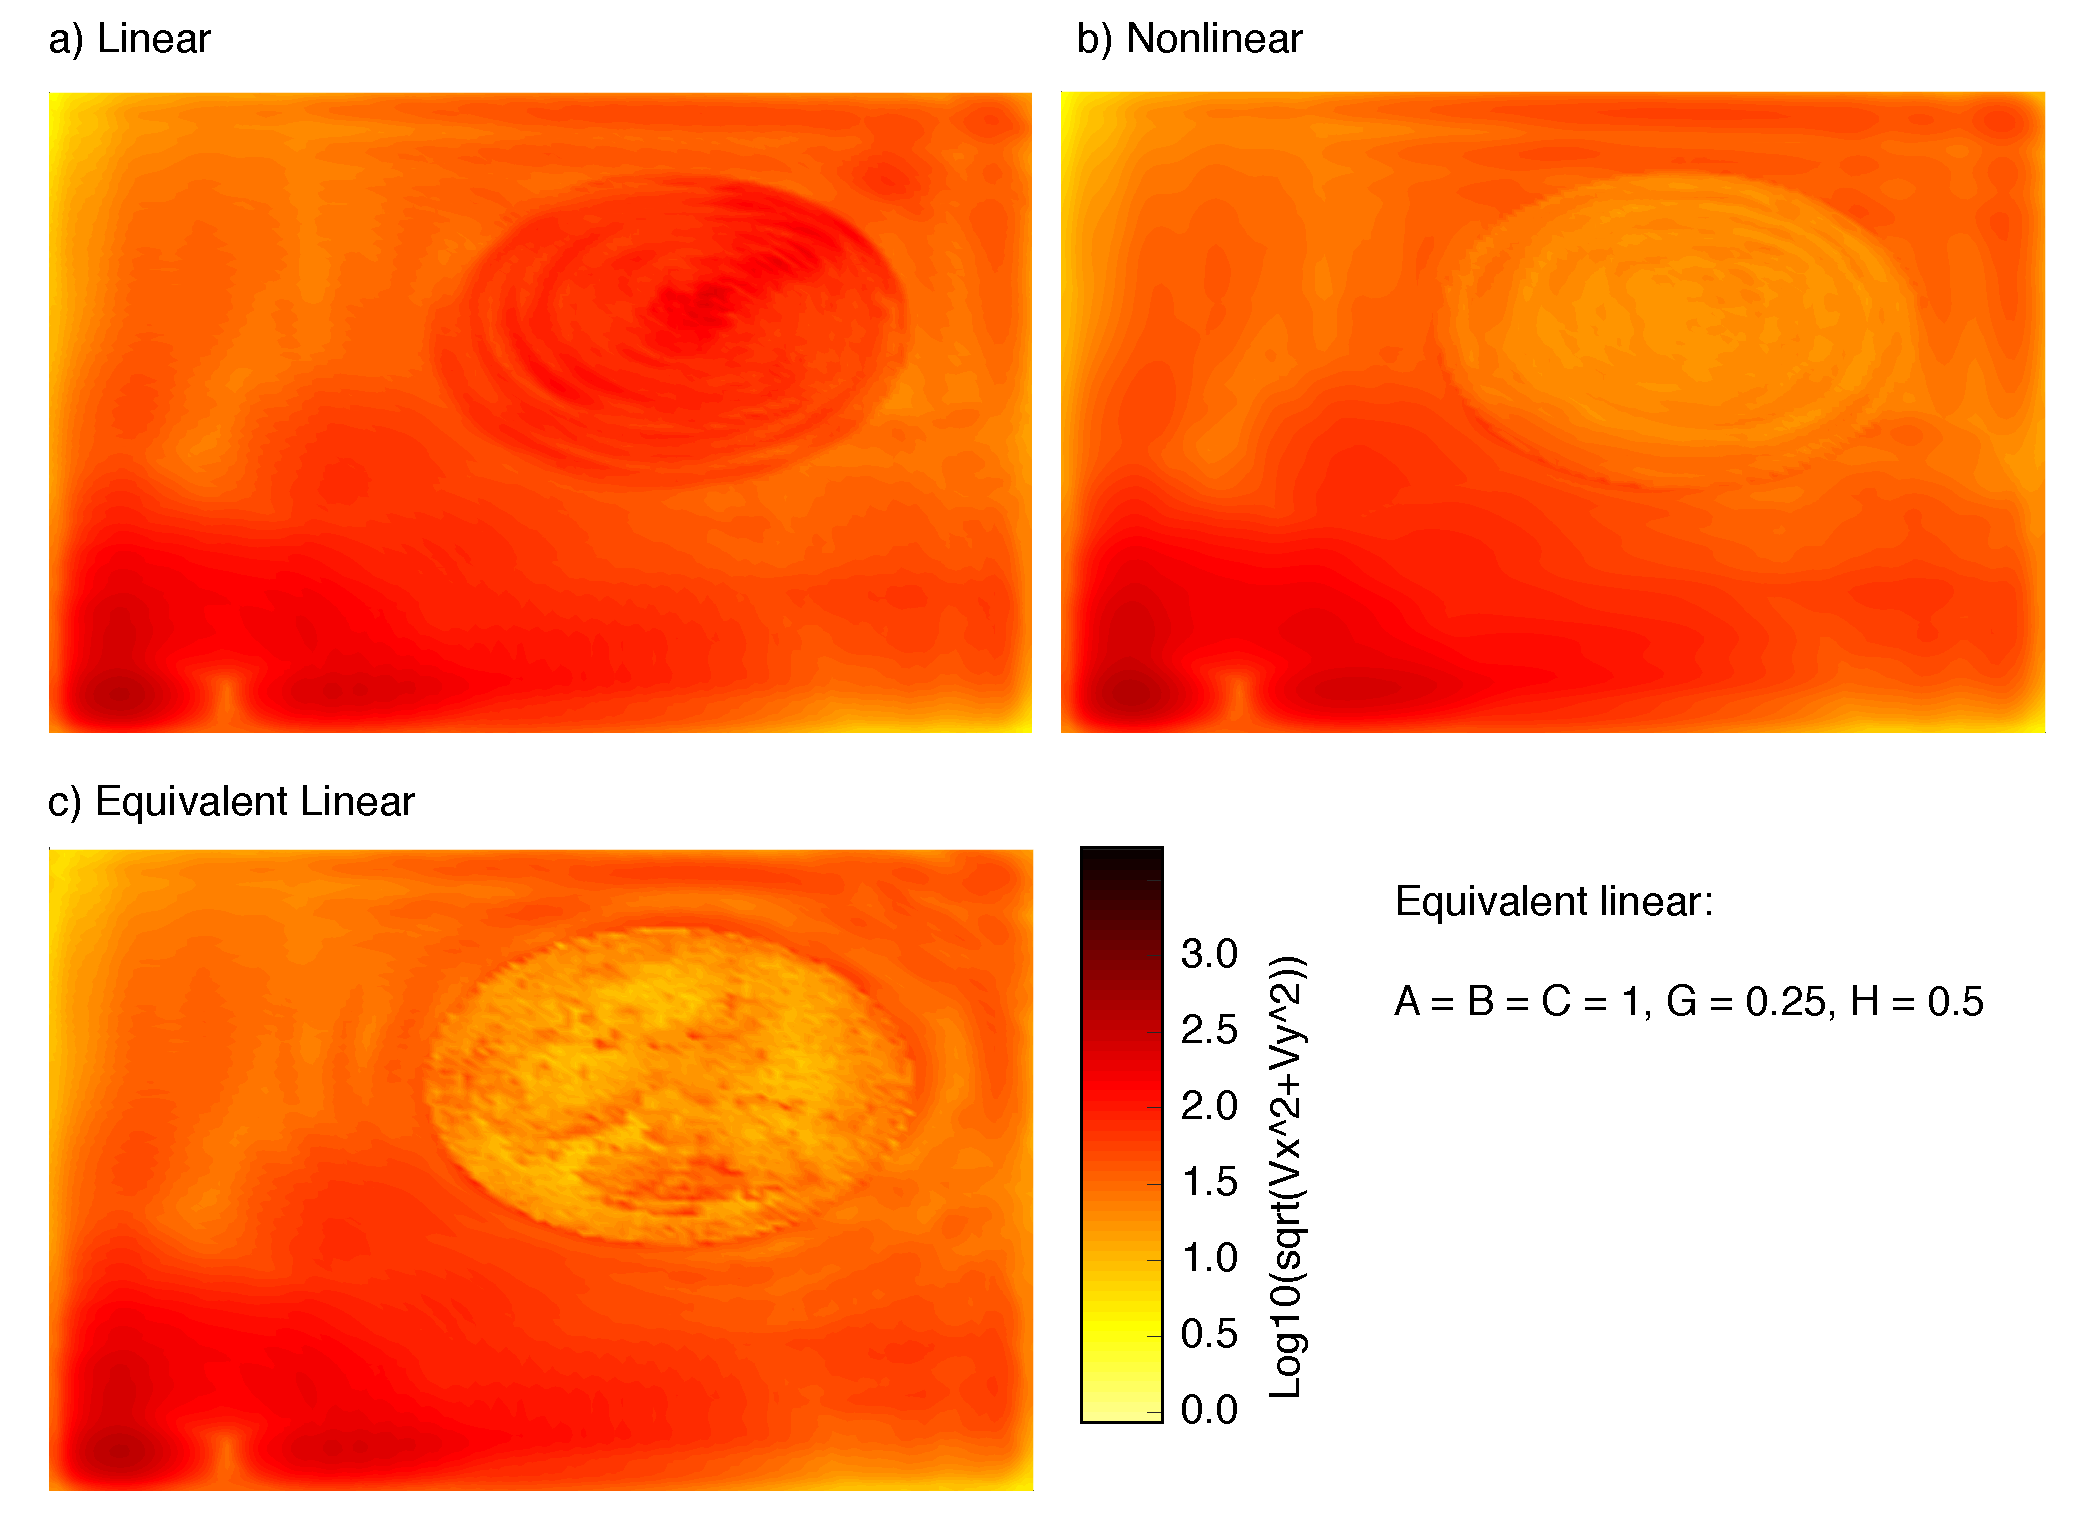
\includegraphics[width=\textwidth]{figures/pdf/plane_lin_nonlin_eqlin.pdf}
    \caption{Geometric peak ground velocity ($v=max(log10(\sqrt{V_x^2+V_y^2}))$) for linear, nonlinear, and equivalent linear simulation. }
    \label{fig:plane_lin_nonlin_eqlin}
\end{figure}

The unwanted heterogeneity that is imposed into the model make the parameter optimization process very difficult. One method to reduce sharp heterogeneities is smoothing effective strain after each iteration. However, implementation of spatial smoothing in 3D is fairly impractical, therefore, we smooth all elements based on the mean effective strain. The idea is reducing very extreme effective strain levels.  Therefore, the smoothed effective strain is defined as

\begin{equation}
updated \epsilon_{eff} = \frac{mean(\epsilon_{eff})+ 3*\epsilon_{eff}}{4};
\end{equation}
 
Fig.~\ref{fig:plane_pgv_smoothed} shows four different simulation with different level of smoothness of effective strain. We also adjust the damping level to fit the model with nonlinear solution. 

\begin{figure}[H]
    \centering
    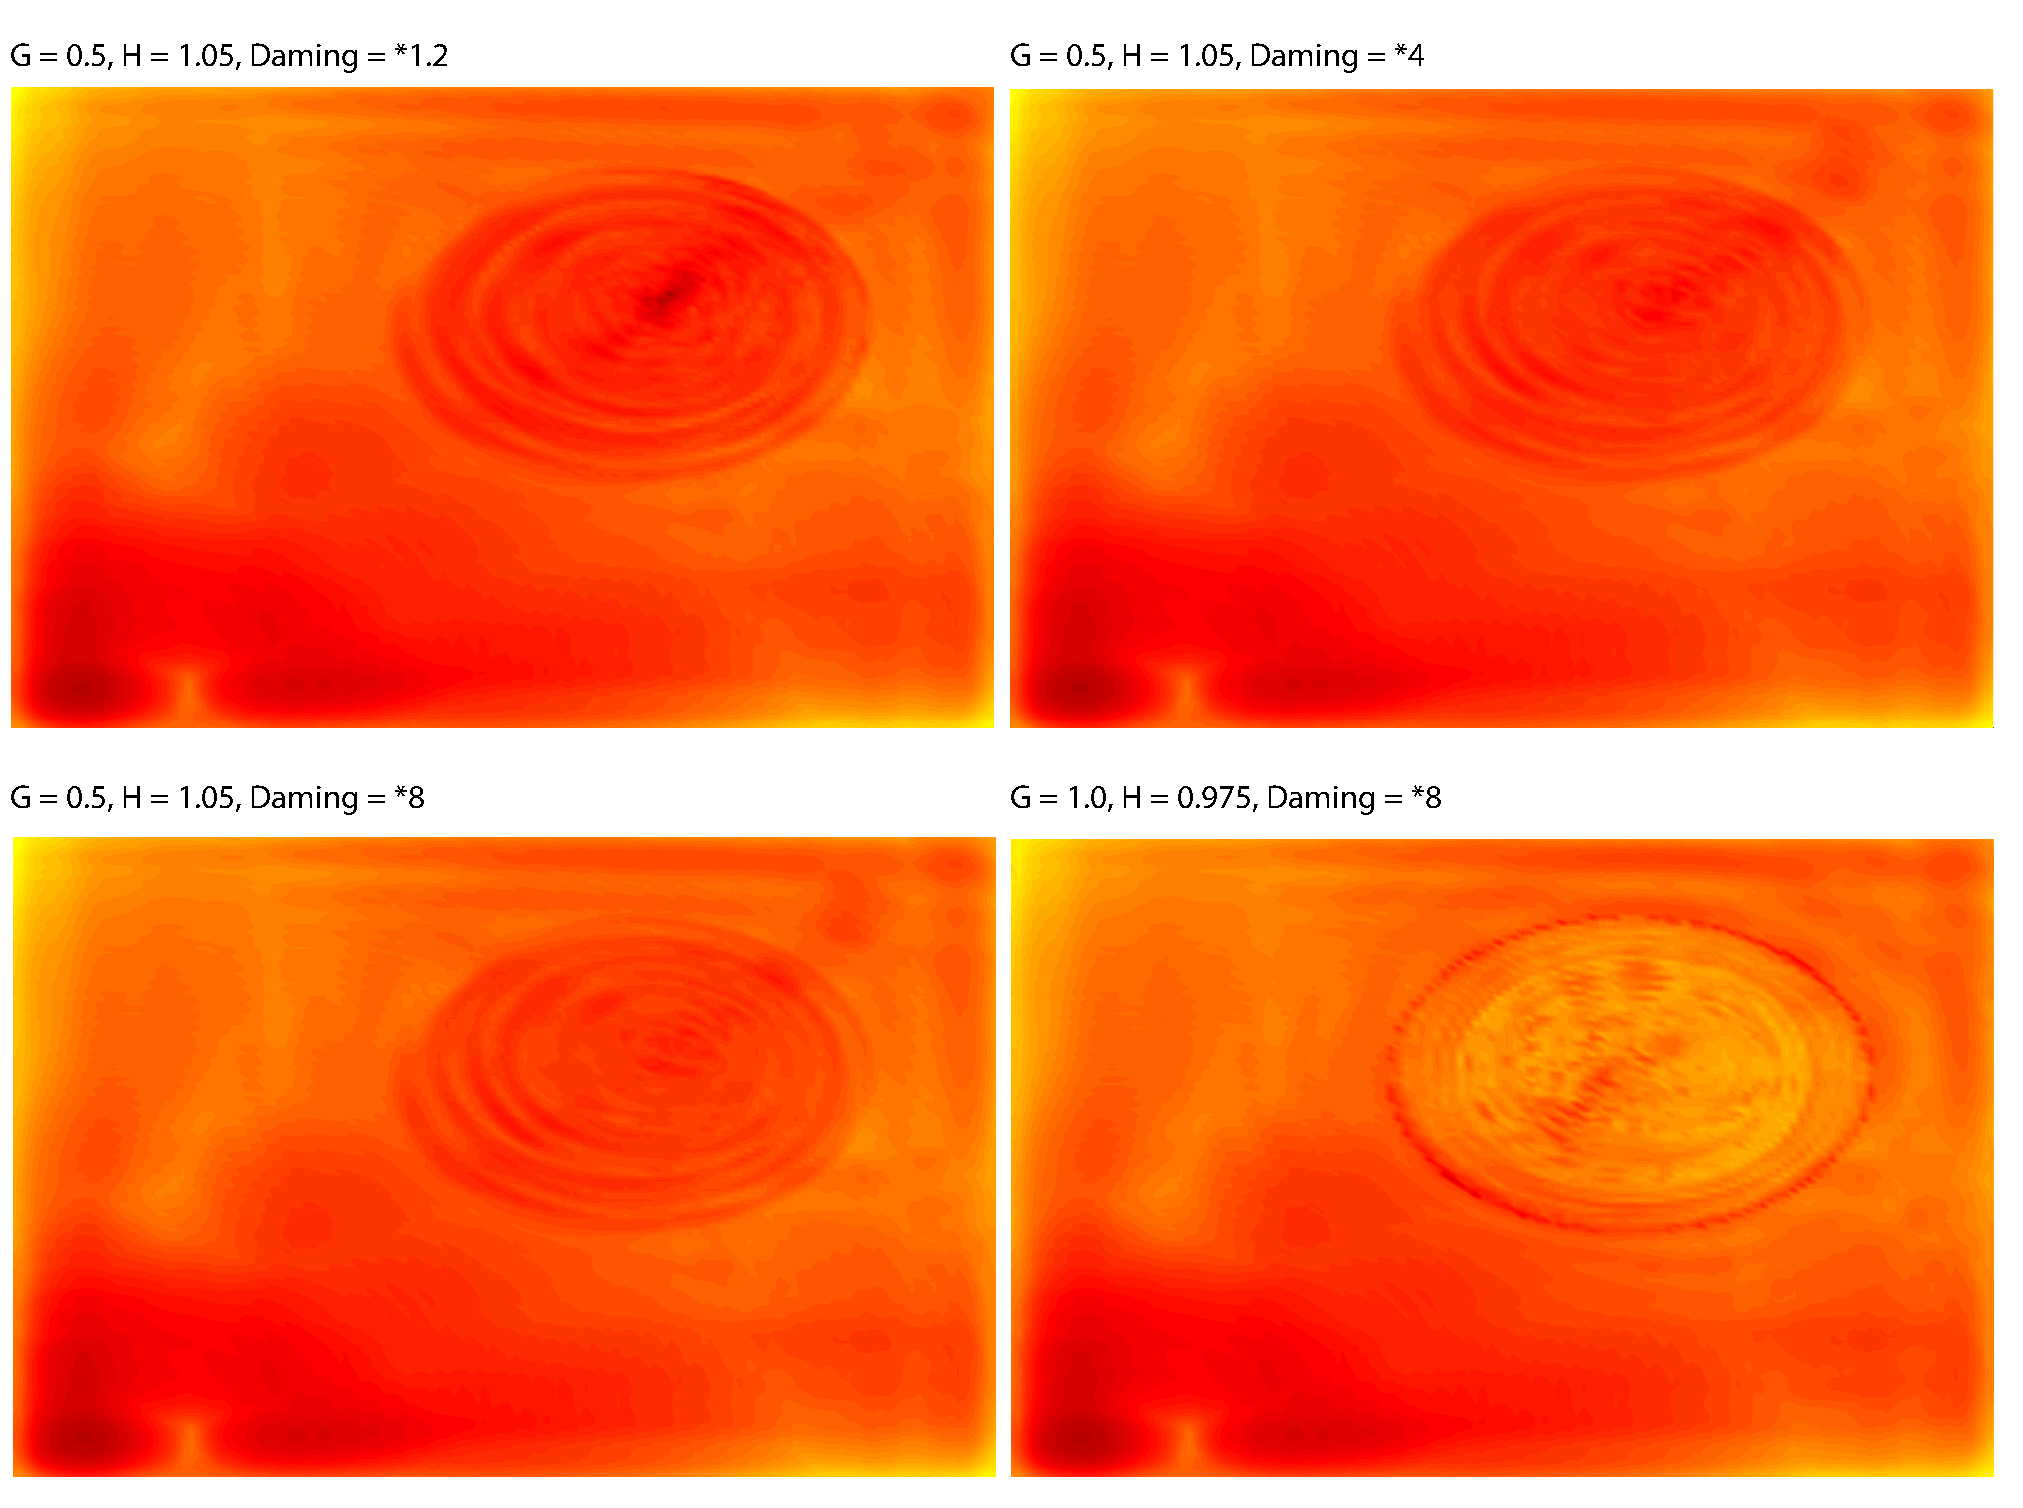
\includegraphics[width=\textwidth]{figures/pdf/plane_pgv_smoothed.pdf}
    \caption{caption. }
    \label{fig:plane_pgv_smoothed}
\end{figure}


Studying unwanted heterogeneity with idealized basin is very difficult. In the next section we test the application with real heterogenous domain with/without smoothing. 